\newpage\phantom{t}
\section{Evaluation}
\label{sec:eval}

\TODO{try to push this earlier}

In this evaluation we simulate datacenter networks with a variety of
next-generation technologies with a wide variety of workloads. Our high-level
goal is to examine how application completion time changes for these workloads
as we introduce a variety of network and cross-layer optimizations.

\TODO{We find that ...}

\subsection{Methodology}
\label{sec:methodology}

We simulate a datacenter network of \TODO{xxx} racks each consisting of
\TODO{xxx} servers in \TODO{xxx}. Each server is connected to a Top-of-Rack
(ToR) switch with a 10Gbps link with 5ns delay. Each ToR is connected to a new
technology switch (NTS) with a 10Gbps link with 500ns delay.

We simulate the various NTS as follows: \TODO{itemized list...}

We simulate the various workloads as follows: \TODO{itemized list...}

We simulate the various optimizations as follows: \TODO{itemized list...}

\srini{Perhaps we don't need such a large scale simulation. Could we simulate
  just one rack and abstract the others?

  If the goal is to see the impact of ``intermittent'' connectivity on
  applications, could we just take the link to the rack up/down? I guess this
  doesn't model contention across racks (e.g. one-to-one mappings) - perhaps we
  can address this statistically in simulation.}


\newpage\phantom{t}
\begin{figure}[t!!!]
\centering
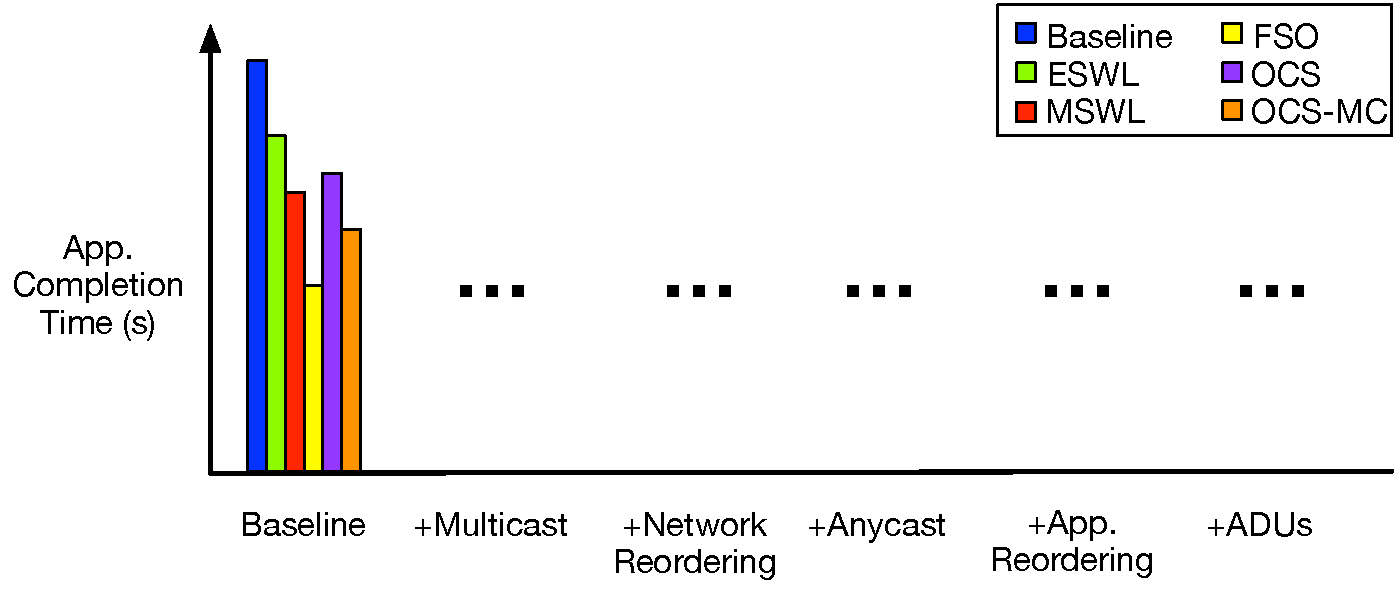
\includegraphics[width=0.47\textwidth]{figures/eval/map_red}
\caption{MapReduce-style Workload.}
\label{fig:eval_MR}
\end{figure}

\subsection{MapReduce Workload}
\label{sec:eval_MR}

\TODO{TODO}





\begin{figure}[t!!!]
\centering
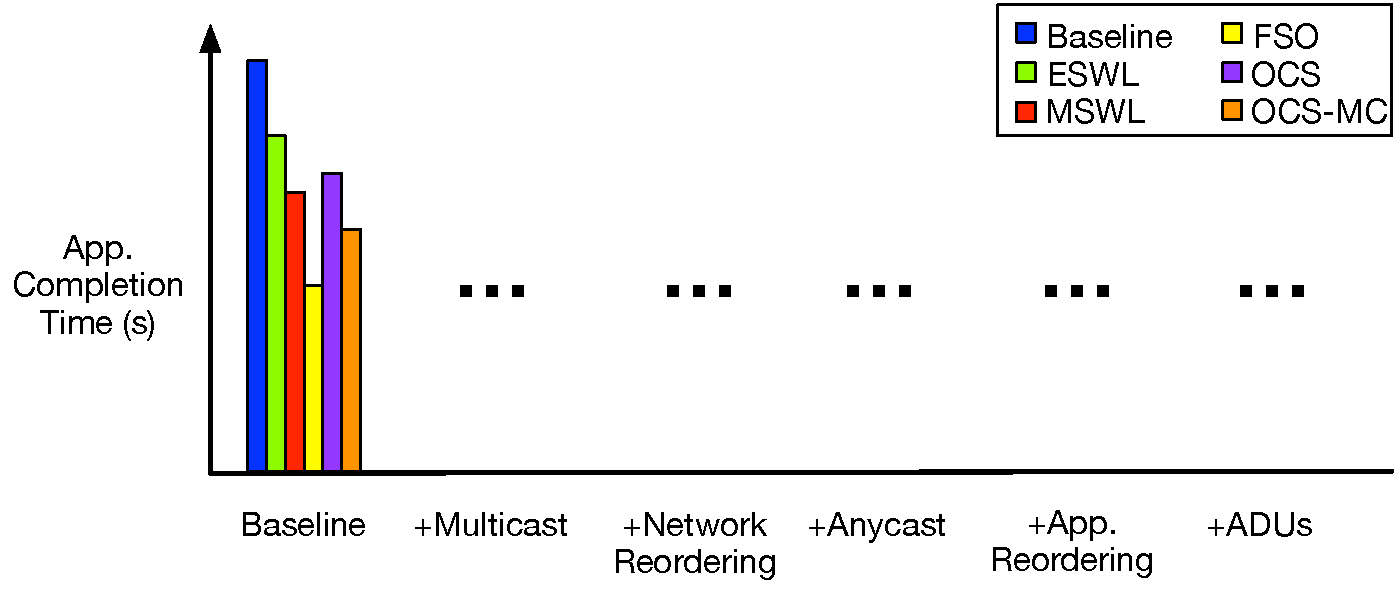
\includegraphics[width=0.47\textwidth]{figures/eval/map_red}
\caption{DFS-style Workload.}
\label{fig:eval_DFS}
\end{figure}

\subsection{DFS Workload}
\label{sec:eval_DFS}

\TODO{TODO}





\newpage\phantom{t}
\begin{figure}[t!!!]
\centering
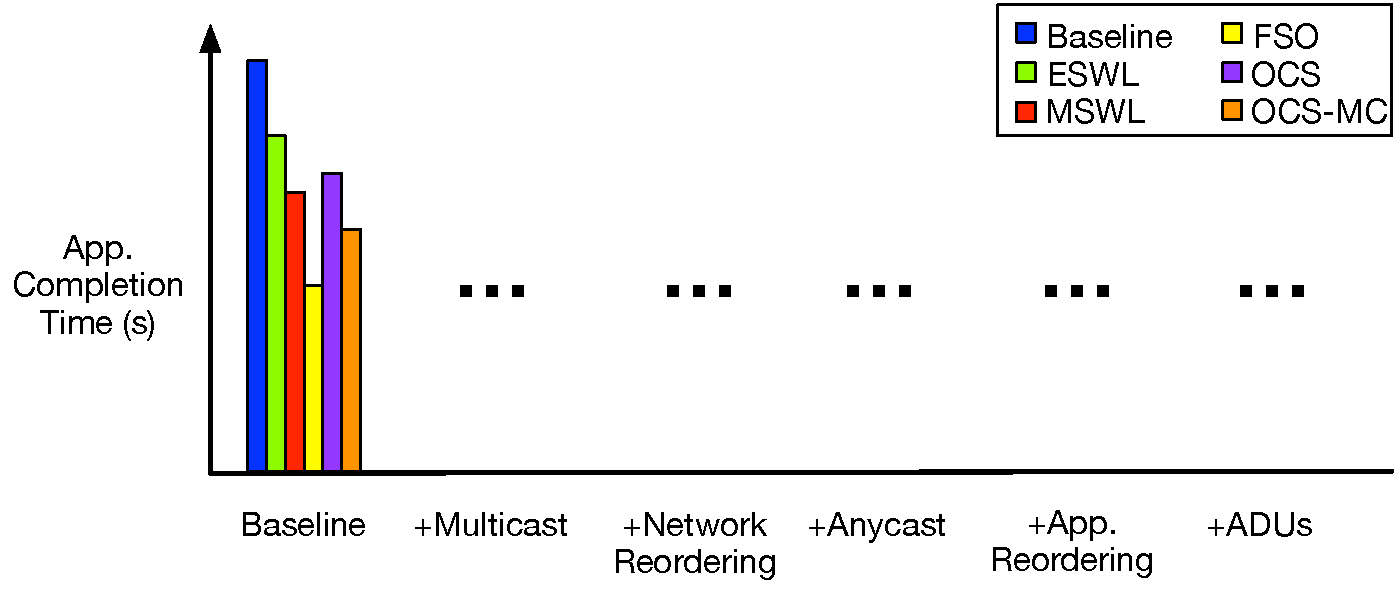
\includegraphics[width=0.47\textwidth]{figures/eval/map_red}
\caption{VM Migration-style Workload.}
\label{fig:eval_VM}
\end{figure}

\subsection{VM Migration Workload}
\label{sec:eval_VM}

\TODO{TODO}







\begin{figure}[t!!!]
\centering
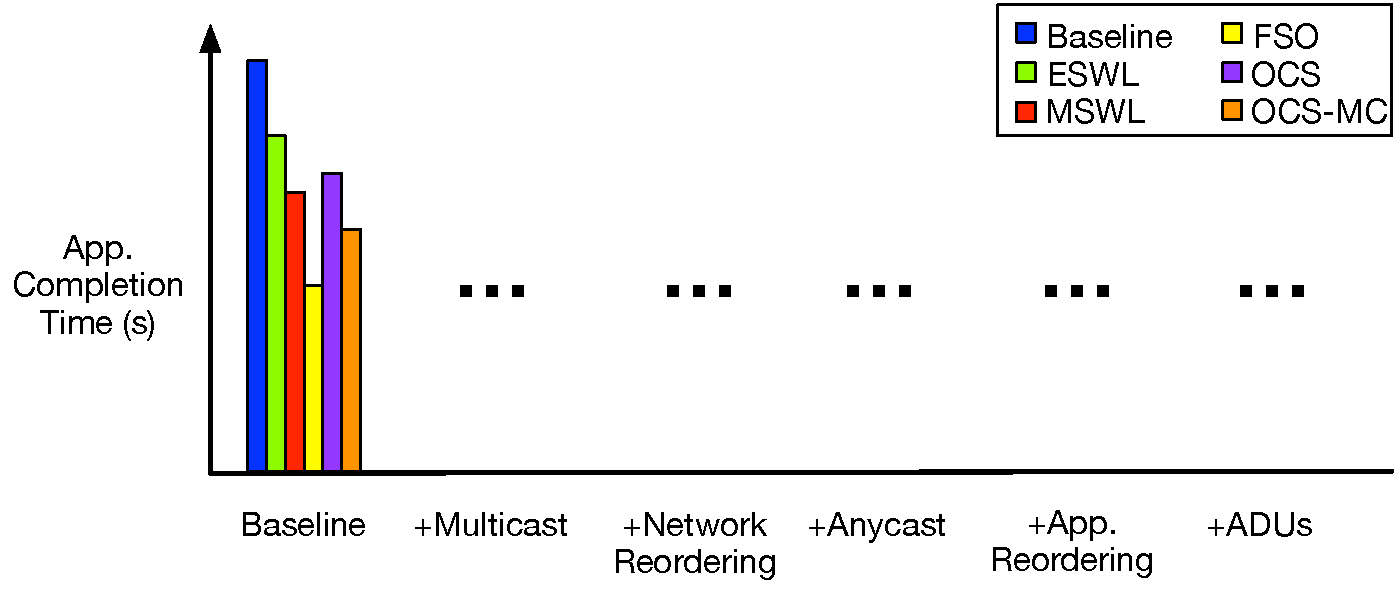
\includegraphics[width=0.47\textwidth]{figures/eval/map_red}
\caption{Search-style Workload.}
\label{fig:eval_search}
\end{figure}

\subsection{Search Workload}
\label{sec:eval_search}

\TODO{TODO}





\newpage\phantom{t}
\begin{figure}[t!!!]
\centering
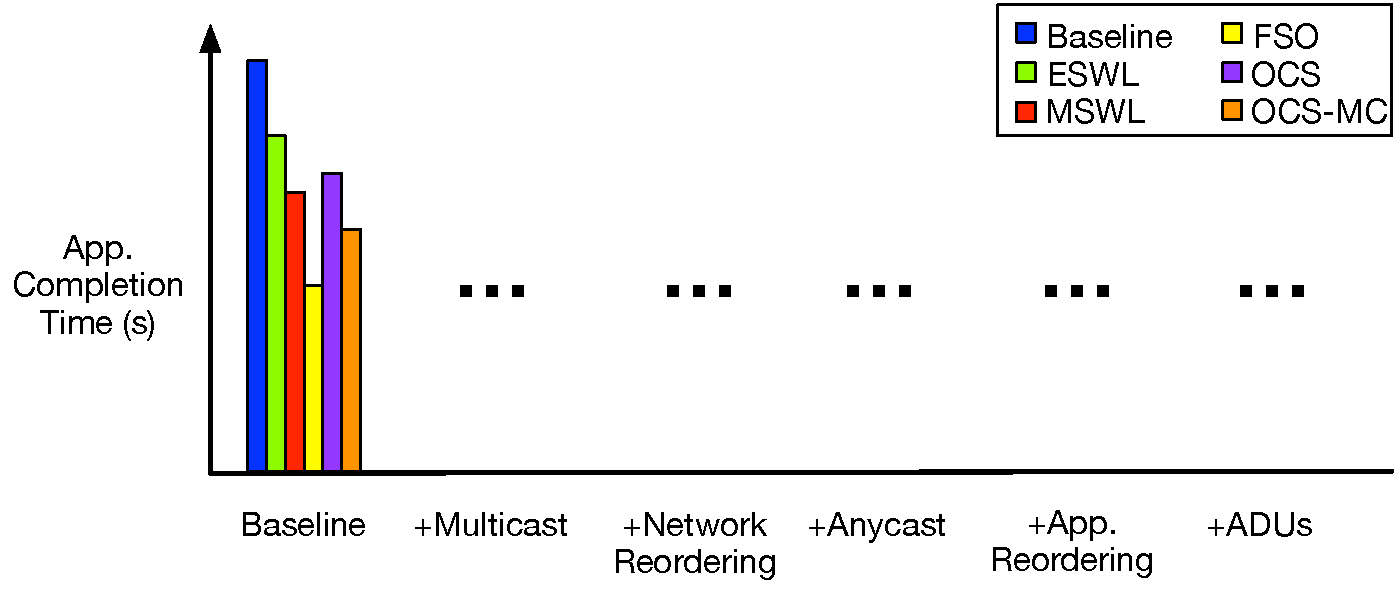
\includegraphics[width=0.47\textwidth]{figures/eval/map_red}
\caption{Combined VM Migration and Search Workload.}
\label{fig:eval_combined}
\end{figure}

\subsection{Combined Workload}
\label{sec:eval_combined}

\TODO{TODO}

